\documentclass[11pt]{article}
% A short summary of the Ontologizer for readers new to the project,
% answering a reviewer's request for: what the method does, what it is for,
% what it assumes and why, how it works, and how it compares with existing
% steering methods. Kept in plain language on purpose: every term is defined
% where it first appears, and project vocabulary from findings.tex is
% avoided (in particular "label" is not used for a classifier's choice;
% it means a ground-truth label). Covers both substrates: GPT-2 results come
% from the headline branch's diagnostics (docs/OVERVIEW.md there), SONAR
% results from findings.tex; change numbers at their source first.
\usepackage[biblatex]{flockpaper}
\usepackage[backend=biber,style=numeric,sorting=none]{biblatex}
\addbibresource{refs.bib}

\title{Unsupervised Steering Vectors from Learned Classifiers:\\
A Summary}
\author{%
  \begin{tabular}[t]{@{}l@{\hspace{2em}}l@{}}
    Keira Wiechecki & Lamb Wakefield \\[2pt]
    \mutedlabel{Wakaru \textperiodcentered{} kaw504@nyu.edu} &
    \mutedlabel{Flock Capital \textperiodcentered{} lamb@flock.holdings} \\[9pt]
    Jade Zaslavsky & vmfunc \\[2pt]
    \mutedlabel{Wakaru \textperiodcentered{} jadeofnameless@gmail} &
    \mutedlabel{Flock Capital \textperiodcentered{} celeste@linux.com}
  \end{tabular}}
\date{\today}

\begin{document}
\maketitle

Checking a model for a hidden goal, or for a concept no one thought to
name, means finding the model's internal variables without anyone
labeling them first. This summary describes a method built for that and
says plainly where it stands: it describes a network's internal state
compactly enough for the network to run on, but editing that description
steers the network no more specifically than editing arbitrary categories
of the same state would, and past the first round the variables it finds
are not the same from one training run to the next. Until both change,
they cannot be named or relied on.

\section*{What the method does}

The method, which we call an \emph{Ontologizer}, rewrites a neural
network's internal representation at one point as a short list of
discrete choices, and rebuilds the representation from them. It is made of
small classifiers. Each classifier sorts every input into one of $k$
categories, and each category stores one vector; the input is rebuilt as
the sum of the vectors its categories select. In the models described here
there are 5 rounds of 32 classifiers with 32 categories each, so an input
is described by 160 choices --- 800 bits --- plus one number per round
giving its overall size. Nothing is labeled: classifiers and vectors are
learned only by asking the rebuilt representation to match the original.

Because a classifier's categories are mutually exclusive, changing one
classifier's choice for an input --- from category $j$ to category $j'$ ---
swaps one stored vector for another. That swap is the steering move the
method is built around: it moves the representation from $j$ to $j'$ along
one axis the method found, and the result is always another valid
description, so the edited representation stays within the range the
network normally sees.

We study two representations. The main one is GPT-2 small's internal
state after its first eight blocks~\cite{radford2019}, on web text: there the
rebuilt state can be put back into the running model, so we can measure
how much of the model's behavior survives. The second is SONAR sentence
embeddings~\cite{sonar}: a fixed-length vector per text, here the opening
of a web document (SONAR is built for sentences), that can be decoded
back into a short paraphrase, which makes a steered embedding readable.

\section*{What it is for}

Watching what a model does cannot settle what it is trying to do: a model
can behave differently when it believes it is being
trained~\cite{greenblatt2024}. Settling it means reading the model's
internal state, including concepts no one has named.

To steer a model is to change its internal state so that it behaves
differently in a chosen way. A standard method is a
\emph{steering vector}: average the representations of examples with a
property, subtract the average of examples without it, and add the
difference to new inputs~\cite{rimsky2024}; a single contrasting pair of
prompts can be enough~\cite{turner2024}. This often works, though not for
every property, and someone who already suspects the property exists
must supply contrasting examples of it. Supervised steering, and the
linear probe that detects a property the same way, can therefore confirm
a concept someone suspects but cannot find one nobody does.

Sparse autoencoders (SAEs) find features without labels: each input is
described by a few active features out of thousands~\cite{bricken2023,
gao2024}. But each feature is an isolated direction that is either on or
off, with no stated alternatives. A feature can stay off on inputs that
have it, because a more specific feature has taken over its
direction~\cite{chanin2025}, so its silence says little; features split
as the dictionary grows~\cite{bussmann2025}; and adding a feature
direction can push the representation anywhere. On a recent steering
benchmark, prompting, fine-tuning and the averaged difference each beat
them~\cite{wu2025axbenchsteeringllmssimple}.

The methods that win are contrasts between alternatives: a property
against its absence, one value of a \emph{variable} --- a property with
several possible values, such as a text's topic --- against another. The
goal is steering vectors that need no labels but keep that shape: each
one a move between named alternatives, found together with the contrast
it moves along. Steering can then test the method, but only against a
baseline: a swap that moves the model's behavior the way the categories
predict shows that the variable matters to the model only if it does
better than swaps between arbitrary categories of the same state. On
both representations it does not yet do better (see below).

\section*{What it assumes, and why that is acceptable}

\begin{enumerate}
\item \textbf{A representation is mostly a sum of a few categorical
choices, plus a remainder that later rounds describe.} Much of language is
categorical --- which token, which syntactic role, which topic --- and
describing a remainder in successive rounds is how residual vector
quantization works in compression~\cite{zeghidour2021}. On GPT-2, 800 bits
per token rebuild the held-out state well enough that, put back into the
model, it recovers 97.5\% of the next-token loss that replacing the state
with its average would cost.
\item \textbf{The classifiers act as roughly independent factors.}
Independence is what lets a few small choices cover many combinations. On
GPT-2 the information shared between two classifiers' choices is 0.27 bits
in the first round and 0.02 bits by the third, against about 5 bits in
each choice.
\item \textbf{The network tolerates running on the description.} If it did
not, editing the description would mean nothing. Beyond the 97.5\%
recovery, swapping one classifier's choice changes GPT-2's next-token
distribution by only 0.001--0.06 nats.
\item \textbf{The categories can be named.} Partly true. On GPT-2, a judge
model shown a description of a first-round category tells its most
typical members from distractors with a score of 0.91, where 0.5 is
chance --- but 0.65 for randomly chosen members and 0.55 for members near
the category's edge, and it is at or near chance in the fourth and fifth
rounds even on the most typical members. Even in the first round, where
29--31 of the 32 classifiers track which token is present, a rule that
sees only the current token's identity beats the judge on single
categories (0.75 vs.\ 0.69 when each classifier has its own block of
coordinates, 0.74 vs.\ 0.71 with direct vectors).
On sentence embeddings, the strongest classifier sorts by topic and genre
(crime news, legislation, encyclopedic description, and so on).
\item \textbf{The categories are a property of the data, not of the
training run.} This has \emph{not} held. Two runs from different random
starts reconstruct equally well, but on both representations only the
first round's classifiers recur; later rounds differ from run to run.
\end{enumerate}

\section*{How it works, intuitively}

\begin{center}
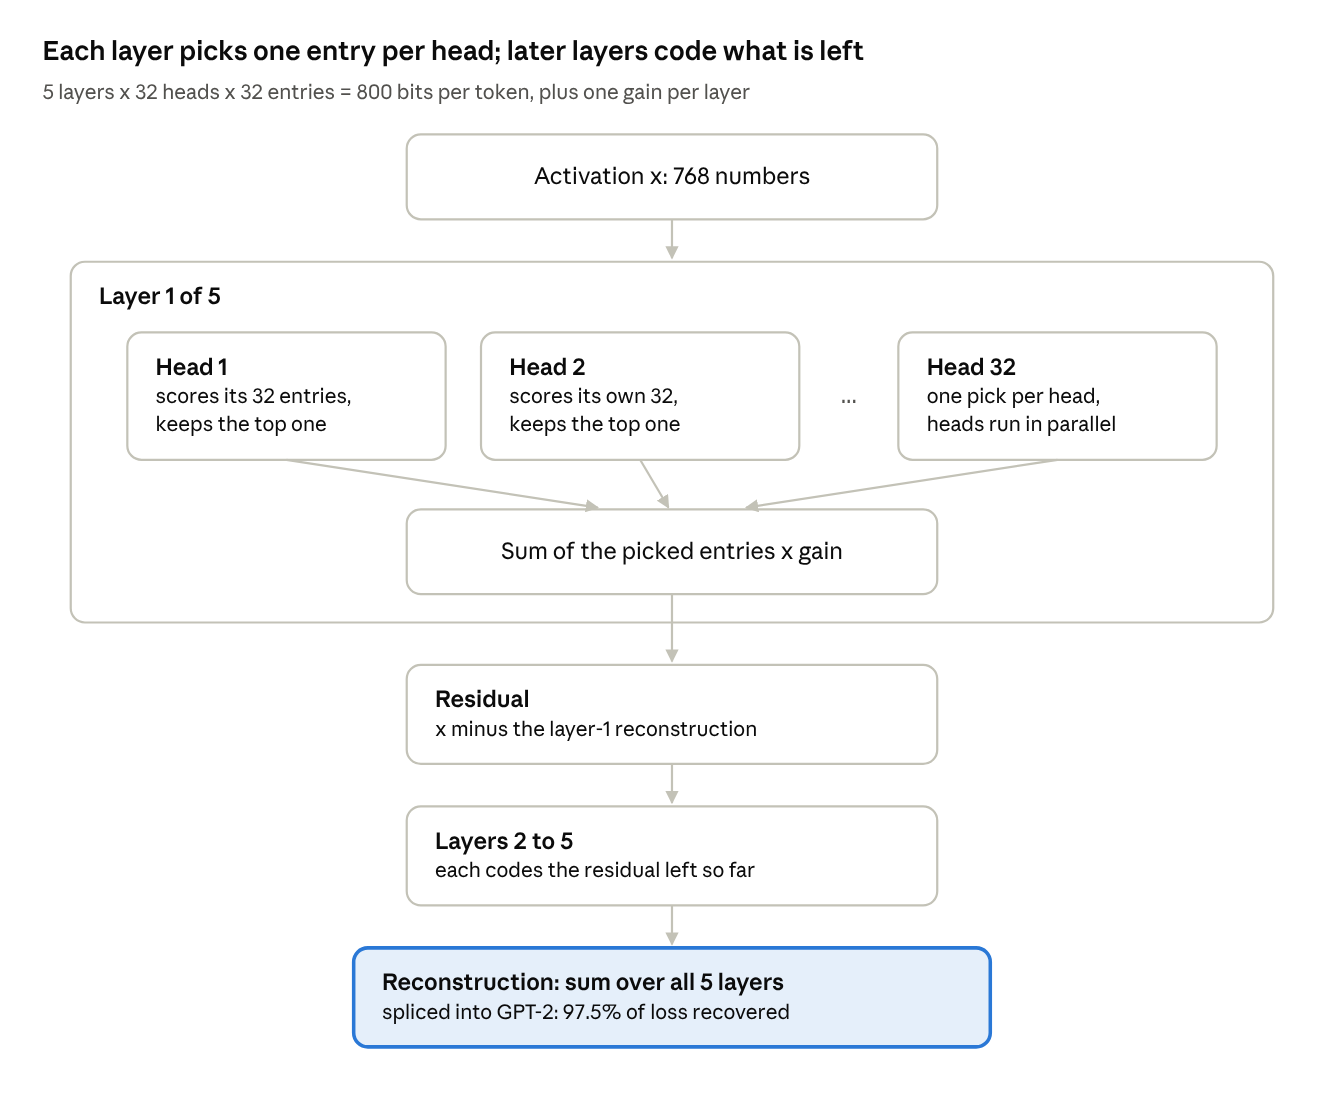
\includegraphics[width=0.78\linewidth]{figures/overview_diagram.png}
\end{center}

Think of describing a token by answering a fixed list of multiple-choice
questions, where the questions and the answers are learned. In the first
round, 32 classifiers each pick their best category in parallel, and the
picked vectors are summed and scaled to the size of what they explain. The
next round sees only what the first got wrong, and describes what
remains; five rounds in all. Training uses hard
choices in the forward pass and soft ones when computing gradients (a
straight-through estimator). The design is a residual quantizer in which
each round adds up vectors picked from several
sets~\cite{zeghidour2021,babenko2014} (product
quantization~\cite{jegou2011} is the case where each set covers its own
coordinates) --- the compression literature's closest relative --- used
not for compression but so that every choice can be read and swapped. The
same kind of quantizer has been used to turn SONAR embeddings into
discrete codes for a language model that writes in
them~\cite{lcmteam2024largeconceptmodelslanguage}.

\section*{How it compares with existing methods}

\textbf{Against supervised steering --- the comparison that matters.}
Three tests so far, none of them yet the decisive one.
\begin{itemize}
\item \emph{Swaps are specific, but so are arbitrary categories (GPT-2).}
Swapping a token's category from $j$ to $j'$ moves the model's output
toward $j'$'s typical output: among 31 alternatives, $j'$ ranks 3.5--6 on
average, and still 5--8 at four times the step, where a random step of the
same size ranks 14--18 (one classifier each in the first, third and fifth
rounds). But categories made by sorting each state by which of 32 random
directions it points along most, with nothing learned, steer just as
specifically in every round (mean rank 0.21--1.69 across the five rounds
against 0.56--1.37 for learned categories, on 8 classifiers per round).
Specificity shows that the state can be steered along any way of dividing
it, not that the method's categories mean anything.
\item \emph{Language (sentence embeddings).} Forcing one of the method's
categories moved decoded text toward a target language 0.64 times as far
as the supervised difference-of-means vector did, and 4 times as far as
a linear-probe direction. All methods, supervised included, damaged
unrelated content about as much as a random step of the same size.
\item \emph{Reaching its own categories (sentence embeddings).} For each
category we fitted the two standard supervised vectors --- difference of
means and a linear probe --- using the method's own assignments as labels
(a generous baseline: it already knows the answer), and gave every
direction the same step. The soft version's own direction reached its
category on 75\% of inputs, against 46--47\% for the supervised vectors;
the hard multi-round version's reached only 37\%, against 91--94\%, so its
categories are reachable but its own direction does not point at them.
Arbitrary categories are just as reachable: on an untrained 5-round model,
the supervised vectors reach 75\% and 94\% of its random categories (and
the classifiers' own gradients 61--85\%) while disturbing a third as many
other classifiers (22\% vs.\ 66\%); on 380 random-direction classifiers of
32 categories, swapping category averages reaches 78\% and the supervised
or projection directions reach 87--100\% while disturbing 30--32\%.
\end{itemize}
The decisive test --- steering toward externally defined concepts, with
supervised vectors fitted to those concepts' labels, SAE features and the
method's swaps scored by the same judge for the concept, for staying on
task and for fluency, each method at its best tuned strength, as in
AxBench~\cite{wu2025axbenchsteeringllmssimple} --- has not been run.

\textbf{Against SAEs on steering.} On sentence embeddings, at each model's
own step size, a feature of a standard SAE (32 active per input) takes
effect on 46--50\% of inputs and the multi-round method on 8--19\%, both
disturbing other features or classifiers about as much as a random step;
a one-round version of the method takes effect on 41\% while disturbing
1.4\% of its other classifiers, against 18\% for a random step. On GPT-2
only removal has been compared: setting one classifier to its average
choice everywhere costs 0.02--0.075 nats, removing one SAE feature where
active 0.055.

\textbf{Against SAEs on reconstruction (a precondition, not the goal).}
Steering through a description only means something if the model runs on
it.
\begin{center}\small\setlength{\tabcolsep}{4pt}
\begin{tabular}{@{}llrr@{}}
\toprule
\begin{tabular}[b]{@{}l@{}}GPT-2 small, after 8 blocks,\\held out\end{tabular}
& per-token code
& \begin{tabular}[b]{@{}r@{}}unexplained\\variance\end{tabular}
& \begin{tabular}[b]{@{}r@{}}loss\\recovered\end{tabular} \\
\midrule
Ontologizer, 32 categories (10M) & 800 bits + 5 numbers & 0.217 & 97.0\% \\
Ontologizer, 32 categories (40M) & 800 bits + 5 numbers & 0.195 & 97.6\% \\
Ontologizer, 32 categories, concat. & 800 bits + 5 numbers & 0.186 & 97.5\% \\
Ontologizer, 64 categories, concat. & 960 bits + 5 numbers & 0.164 & 97.9\% \\
SAE, 32 active features & 32 indices + 32 numbers & 0.189 & 96.2\% \\
SAE, 128 active features & 128 indices + 128 numbers & 0.116 & 98.6\% \\
\bottomrule
\end{tabular}
\end{center}
Both on the same 10M-token training cache (97.0\% vs.\ 96.2\%) and after
one pass over 40M tokens (97.5--97.6\%), the 800-bit description recovers
more of the model's loss than the 32-feature SAE, so its errors fall where
the model cares less, though with the SAE's 32 numbers rounded to about 5
bits each (556--588 total bits) the SAE leads on unexplained variance per
bit. Giving each round of the concatenated-head model its own output
projection instead of one shared across all five rounds cuts unexplained
variance from 0.186 to 0.169 (97.3\% to 97.7\% loss recovered) and drops
cross-round coupling of the same classifier slot from 97\% to 6\%. On sentence embeddings, 1900 bits of choices and the
per-round sizes leave 15\% of the variance unexplained, and 16\% with the
sizes fixed. A standard SAE whose description is held to the same 1900
bits, about 1200 saying which 160 features are active and the rest for
their 160 numbers, leaves at least 24\% however those numbers are
rounded. But an SAE trained with a weaker sparsity penalty, its numbers
rounded coarsely and each feature's activity coded by how often it fires,
leaves 13\% at 1900 bits: its features fire unevenly, which makes the
list of active ones cheap to send, while the method's categories are used
evenly and leave nothing to save.

\section*{What we can claim}

On both representations the method describes the network's state with a
small set of discrete choices about as accurately as a sparse autoencoder
that also sends continuous numbers (more accurately than the standard
kind at the same number of bits, though not than every kind), and on
GPT-2 the model runs on that description with little loss. Swapping
one choice moves the model's output specifically toward the new
category, though swapping between arbitrary categories does too. Some
categories can be named: on GPT-2, a first-round category from its most
typical members (0.91, where 0.5 is chance), though a token-identity rule
beats the judge on single first-round categories (0.74--0.75 vs.\
0.69--0.71) and combining two first-round categories adds +0.10 on
concatenated heads (0.69 to 0.78, mostly from token identity) and +0.01
on direct vectors (0.71 to 0.72); on
sentence embeddings, a topic-and-genre classifier that recurs in every
run. Whether the categories are in general easier to interpret than SAE
features, whether they steer better than arbitrary categories, and
whether swapping them steers better than supervised vectors toward
concepts a user cares about, is not established.

\section*{What does not work yet}

\begin{itemize}
\item \textbf{The classifiers past the first round are not reproducible.}
This is the main open problem, not a detail. Two runs reconstruct equally
well but agree on almost none of these classifiers, on both
representations, so reconstruction quality cannot reveal the failure. A
classifier that differs on every run cannot be named, an audit could not
rely on it, and a goal defined in terms of it would not keep pointing at
the same thing once the model is retrained.
\item \textbf{Categories are named from their extremes.} Descriptions fit a
category's most typical members, not its ordinary ones, the failure
automated description shows when it sees only the strongest
examples~\cite{paulo2025}, and the deeper
rounds cannot yet be named at all, though changing them does change the
model's output.
\item \textbf{Swaps do not yet beat arbitrary categories.} On both GPT-2
and sentence embeddings, categories made from random directions or an
untrained model steer their own cells as specifically as the learned ones,
so the case for the deeper rounds rests on reconstruction alone.
\item \textbf{Steering through the input is not targeted.} On sentence
embeddings, pushing an input toward one category changes other
classifiers' choices about as much as a random push of the same size.
Swaps made on the description itself do not have this problem.
\end{itemize}

\section*{Next}

Reproducibility comes first: making the classifiers reproducible, or
identifying the ones that are. Theory shows that reconstructing individual
inputs cannot identify discrete or continuous factors without structural
constraints matched to the data or paired views such as adjacent
sentences~\cite{locatello2019,hillar2015,allman2009,udr2020,pcl2017,slowvae2021,locatello2020,ivae2020,zimmermann2021}.
On 44.1M consecutive sentence embeddings, a linear predictor from one
sentence explains only about 10\% of the next sentence's variance
(unexplained variance 0.896), and while adjacent sentences point in
similar directions (cosine discrimination 0.923), existing classifiers
switch categories on 92.2--98.1\% of adjacent pairs; directly penalizing
category changes across adjacent sentences collapses the penalized
classifiers to 0.04--0.09 bits, pointing instead to a hinged
conditional-entropy bound that turns off once transitions between a
classifier's categories are sparse.

The test the method then needs is AxBench-style steering toward
externally defined concepts~\cite{wu2025axbenchsteeringllmssimple}:
difference-of-means vectors from labeled examples, SAE features and the
method's swaps, each at its best tuned strength, scored by a judge for
the concept, for staying on task and for fluency, plus detection against
a linear probe. Initial runs on Gemma~3 1B and Gemma~4 A4B, using
mean-squared error with a small uniformity penalty and per-round output
projections, are underway toward that evaluation.

\printbibliography

\end{document}
